\documentclass[a4paper,12pt]{report}

\usepackage[utf8]{inputenc}
\usepackage[a4paper,margin=24mm]{geometry}
\usepackage[skip=10pt plus1pt, indent=20pt]{parskip}
\usepackage[colorlinks=true,allcolors=blue,urlcolor=magenta]{hyperref}

\usepackage{caption}
\usepackage{indentfirst,setspace,subcaption}
\usepackage{amsmath,amssymb,graphicx,xcolor,url}
\usepackage{fancyhdr,tocbasic,titlesec,minted,listings}
\usepackage{algorithm}
\usepackage{algpseudocode}

\renewcommand{\thesection}{\arabic{section}}

\renewcommand{\thesection}{\arabic{section}}
\renewcommand{\listoflistingscaption}{Source code}

\newcommand{\codeimport}{\inputminted[breakanywhere=true,breaklines=true]}


% Code highlighting
\usemintedstyle{one-dark}
\setminted{frame=lines,
  framesep=2mm,
  baselinestretch=1.2,
  fontsize=\footnotesize,
  linenos,
  breakanywhere,
  breaklines,
  mathescape
}

% Header and footer styling
\pagestyle{fancy}
\setlength{\headheight}{18pt}
\fancyhf{}
\fancyhead[R]{\nouppercase\rightmark\hfill~Project 02: Hashiwokakero}
\fancyfoot[C]{\hfill\thepage\hfill}

% TOC styling
\DeclareTOCStyleEntry[
  indent=12pt,
  level=1
]{largetocline}{section}

% Title page data
\title{Project 02: Hashiwokakero}
\author{\begin{tabular}{r c}
  Ngo Nguyen The Khoa & 23127065\\
  Bui Minh Duy       & 23127040\\
  Nguyen Le Ho Anh Khoa      & 23127211\\
\end{tabular}}
\date{April 5, 2025}

\begin{document}
\newenvironment{codewithlisting}[2]{
	\begin{listing}[!ht]
		\caption[#1]{#1}
		\label{listing:#2}}{\end{listing}
}


% Title page and TOC
\thispagestyle{empty}
\begin{titlepage}
	\begin{center}
		\makeatletter
		\newcommand{\HRule}{\rule{\linewidth}{0.4mm}}

		\textsc{\LARGE Vietnam National University,\\Ho Chi Minh City}\\[1.5cm]
		\textsc{\Large University of Science}\\[0.5cm]
		\textsc{\Large Faculty of Information Technology}\\[1.5cm]

		{\HRule}\\[1cm]
		{\huge \bfseries \@title}\\[0.5cm]
		{\HRule}\\[2cm]

		\textsc{\large CS14003 --  Introduction to Artificial Intelligence}\\[0.5cm]

		\vfill\vfill\vfill

		{\large \@author}\\[1.5cm]
		{\large \@date}
		\makeatother
	\end{center}
\end{titlepage}

\tableofcontents\thispagestyle{empty}

% Report contents
\pagebreak
\section{Group Information}
\begin{itemize}
  \item \textbf{Subject:} Introduction to Artificial Intelligence.
  \item \textbf{Class:} 23CLC09.
  \item \textbf{Lecturer:} Bui Duy Dang, Le Nhut Nam.
  \item \textbf{Team members:}
        \begin{center}
          \renewcommand{\arraystretch}{1.5}
          \begin{tabular}{|c|l|c|l|}
            \hline
            \textbf{No.} & \textbf{Fullname}     & \textbf{Student ID} & \textbf{Email}                                                         \\\hline
            1            & Ngo Nguyen The Khoa   & 23127065            & \href{mailto:nntkhoa23@clc.fitus.edu.vn}{nntkhoa23@clc.fitus.edu.vn}   \\\hline
            2            & Bui Minh Duy          & 23127040            & \href{mailto:bmduy23@clc.fitus.edu.vn}{bmduy23@clc.fitus.edu.vn}       \\\hline
            3            & Nguyen Le Ho Anh Khoa & 23127211            & \href{mailto:nlhakhoa23@clc.fitus.edu.vn}{nlhakhoa23@clc.fitus.edu.vn} \\\hline
          \end{tabular}
        \end{center}
\end{itemize}

\section{Project Information}
\begin{itemize}
  \item \textbf{Name:} Decision Tree Classifier using Scikit-learn.
  \item \textbf{Developing Environment:} Visual Studio Code (Windows, WSL).
  \item \textbf{Programming Language:} Python.
  \item \textbf{Libraries and Tools:}
        \begin{itemize}
          \item \textbf{Libraries:}
                \begin{itemize}
                  \item \href{https://scikit-learn.org/stable/}{\textbf{scikit-learn:}} Machine learning library for training and evaluating decision tree models.
                  \item \href{https://pandas.pydata.org/}{\textbf{pandas:}} Data manipulation and analysis.
                  \item \href{https://numpy.org/}{\textbf{numpy:}} Numerical operations.
                  \item \href{https://matplotlib.org/}{\textbf{matplotlib}}, \href{https://seaborn.pydata.org/}{\textbf{seaborn:}} Data visualization libraries.
                  \item \href{https://graphviz.org/}{\textbf{graphviz:}} Visualization of decision trees.
                \end{itemize}
          \item \textbf{Tools:}
                \begin{itemize}
                  \item \href{https://git-scm.com/}{\textbf{Git}}, \href{https://github.com/}{\textbf{GitHub}}: Source code version control.
                  \item \href{https://code.visualstudio.com/}{\textbf{Visual Studio Code}}: Code editor for Python, LaTeX.
                \end{itemize}
        \end{itemize}
  \item \textbf{Datasets:}
        \begin{itemize}
          \item \href{https://archive.ics.uci.edu/dataset/17/breast+cancer+wisconsin+diagnostic}{\textbf{Breast Cancer Wisconsin (Diagnostic)}}
          \item \href{https://archive.ics.uci.edu/dataset/186/wine+quality}{\textbf{Wine Quality}}
          \item \href{https://archive.ics.uci.edu/dataset/19/car+evaluation}{\textbf{Car Evaluation}}
        \end{itemize}
\end{itemize}


\pagebreak
\section{Work Assignment Table}
\begin{center}
  \renewcommand{\arraystretch}{1.5}
  \begin{tabular}{|c|p{\dimexpr0.55\linewidth-2\tabcolsep}|r|c|}
    \hline
    \textbf{No.} & \textbf{Task Description}                                                                                                 & \textbf{Assigned to} & \textbf{Rate} \\\hline
    1            & Prepare all three datasets (Breast Cancer, Wine Quality, and Additional) with proper preprocessing and stratified splits. & The Khoa             & 100\%         \\\hline
    2            & Implement and train decision tree models for each dataset with different train/test splits.                               & Minh Duy             & 100\%         \\\hline
    3            & Visualize decision trees using Graphviz.                                                                                  & Anh Khoa             & 100\%         \\\hline
    4            & Evaluate classifiers with classification reports and confusion matrices.                                                  & Anh Khoa             & 100\%         \\\hline
    5            & Analyze impact of tree depth on accuracy (80/20 split, varying max\_depth values).                                        & The Khoa             & 100\%         \\\hline
    6            & Research and integrate additional dataset.                                                                                & Minh Duy             & 100\%         \\\hline
    7            & Conduct comparative analysis across the three datasets.                                                                   & The Khoa             & 100\%         \\\hline
    8            & Visualize and format results (accuracy tables, charts, dataset distributions, etc.).                                      & Anh Khoa             & 100\%         \\\hline
    9            & Write and format final report with all results, insights, and figures.                                                    & Minh Duy             & 100\%         \\\hline
    10           & Ensure overall cohesion, proofreading, and prepare final PDF submission.                                                  & All                  & 100\%         \\\hline
  \end{tabular}
\end{center}

\section{Self-evaluation}
\begin{center}
  \renewcommand{\arraystretch}{1.5}
  \begin{tabular}{|c|p{\dimexpr0.82\linewidth-2\tabcolsep}|c|}
    \hline
    \textbf{No.} & \textbf{Task Description}                                                                  & \textbf{Rate} \\\hline
    1            & Prepare datasets with stratified splits and visualize class distributions.                 & 100\%         \\\hline
    2            & Train and visualize decision tree models on all datasets using multiple train/test splits. & 100\%         \\\hline
    3            & Evaluate decision trees using classification reports and confusion matrices.               & 100\%         \\\hline
    4            & Analyze the impact of decision tree depth on model accuracy.                               & 100\%         \\\hline
    5            & Research and integrate an additional dataset for training and evaluation.                  & 100\%         \\\hline
    6            & Conduct comparative analysis across all datasets.                                          & 100\%         \\\hline
    7            & Create charts, tables, and visualizations to support findings.                             & 100\%         \\\hline
    8            & Write and format the final report with insights and well-organized results.                & 100\%         \\\hline
    9            & Team collaboration and adherence to project schedule.                                      & 100\%         \\\hline
  \end{tabular}
\end{center}


\pagebreak
\input{pages/CNF.tex}

\pagebreak
\section{Algorithms' Implementations}
\input{pages/PySAT.tex}
\input{pages/Astar.tex}
\subsection{Backtracking with DPLL-based SAT Solver}
\noindent The backtracking algorithm used for solving Hashiwokakero puzzles is based on a simplified DPLL (Davis–Putnam–Logemann–Loveland) SAT solver. The puzzle is first encoded into CNF form, and then a recursive backtracking search is employed to find a satisfying assignment of Boolean variables. This approach systematically explores the space of assignments and applies inference rules like unit propagation and pure literal elimination to prune inconsistent paths early, improving efficiency over naïve brute force methods.

\subsubsection{Implementation Details}
\begin{itemize}
	\item \textbf{unit\_propagate():}
	      \begin{flushleft}
		      This function iteratively applies unit clause inference.\\ When a clause has only one unassigned literal, it forces the corresponding variable to satisfy the clause, reducing the search space.
	      \end{flushleft}
	\item \textbf{dpll():}
	      \begin{flushleft}
		      The core recursive backtracking function. It applies unit propagation and pure literal elimination before branching.\\ For each unassigned variable, it tries both True and False values recursively until it finds a satisfying assignment or concludes unsatisfiability.
	      \end{flushleft}
	\item \textbf{solve\_with\_backtracking():}
	      \begin{flushleft}
		      Encodes the puzzle into CNF, calls the DPLL solver, and if a model is found, it validates and extracts the solution using utility functions like \textit{validate\_solution} and \textit{generate\_output}.
	      \end{flushleft}
\end{itemize}

\subsubsection{Inference Techniques} The algorithm integrates classical SAT-solving inference techniques to enhance performance:
\begin{itemize}
	\item \textbf{Unit Propagation:} Forces assignments based on clauses with only one remaining unassigned literal.
	\item \textbf{Pure Literal Elimination:} Assigns values to literals that always appear with the same polarity (positive or negative) across all clauses.
\end{itemize}

\subsubsection{Time and Space Complexity}
\textbf{Time Complexity:} In the worst case, the algorithm explores all possible assignments, resulting in \(O(2^n)\) time complexity, where \(n\) is the number of variables. However, unit propagation and pure literal elimination help prune large portions of the search tree.

\textbf{Space Complexity:} \(O(n+m)\), where \(n\) is the number of variables and \(m\) is the number of clauses. Additional space is used to store the recursive call stack and intermediate assignments during backtracking.

\subsection*{Strengths}
\begin{itemize}
    \item \textbf{High Performance with DPLL:} The backtracking solver, now integrated with the DPLL-based approach, can solve puzzles with impressive speed and efficiency, even for large instances, significantly improving performance over the base version.
    \item \textbf{Scalability in Size:} The DPLL-enhanced solver can handle large puzzle sizes effectively, maintaining high performance across a wide range of problem dimensions.
    \item \textbf{Simplicity of the Base Algorithm:} The core backtracking logic is simple to implement, providing an easy starting point for logic puzzle solving, though the performance of this base approach is not optimal.
\end{itemize}

\subsection*{Limitations}
\begin{itemize}
    \item \textbf{Implementation Complexity with DPLL:} The DPLL-based approach, while offering superior performance, is more advanced to implement and debug. It requires careful handling of SAT-solving techniques like unit propagation and pure literal elimination, which can be error-prone.
    \item \textbf{Base Algorithm Performance:} While the base backtracking algorithm is easy to implement, its performance is poor compared to the DPLL-enhanced version, making it unsuitable for large or complex puzzles.
    \item \textbf{Debugging Difficulty in DPLL:} Debugging issues in the DPLL-based version is more challenging due to its abstract nature, making it harder to trace failures compared to more traditional, step-by-step solvers.
\end{itemize}

\subsection*{Conclusion}
The backtracking solver, when enhanced with the DPLL algorithm, represents a significant improvement in terms of performance and scalability for solving logic puzzles. The DPLL-based approach enables the solver to handle larger problem instances efficiently, achieving impressive speed compared to the base backtracking method. While the base algorithm remains easy to implement and serves as a simple foundation for puzzle solving, its performance is insufficient for more complex problems. On the other hand, the DPLL version, though more advanced and challenging to implement, offers a much more powerful solution.

\input{pages/Brute.tex}

\pagebreak
\section{Algorithms Benchmark}
\subsection{About Test Cases}
\begin{itemize}
    \item \textbf{Test cases description}
          \begin{itemize}
              \item Each map size in (7 × 7), (9 × 9), (11 × 11), (13 × 13), (17 × 17), (20 × 20) has at least 5 test cases with different difficulty levels. (There are also test cases for (3 × 3) and (5 × 5) for brute force algorithm.)
              \item The test cases are generated randomly and the difficulty levels are classified as easy, medium, hard, and very hard with the increasing of crossing edges, the number of islands with high degrees, etc. The results of the tests are shown in the table and figures below. The time is measured in milliseconds (ms) and the peak memory is measured in kilobytes (KB).
          \end{itemize}


    \item \textbf{Challenges}
          \begin{itemize}
              \item \textbf{Generating CNF}
                    \begin{itemize}
                        \item Generating CNF clauses for constraints like `degree constraints' is quite complex and time-consuming. The algorithm needs to consider all possible combinations of edges and nodes to generate the CNF clauses.
                    \end{itemize}
              \item \textbf{Algorithm implementations}
                    \begin{itemize}
                        \item The algorithm is not optimal for large maps, which leads to a long solving time and high peak memory usage.
                        \item The algorithm is not able to solve some test cases with a very high difficulty level.
                    \end{itemize}
          \end{itemize}
\end{itemize}

\subsection{Experiment results}
\begin{flushleft}
    \begin{itemize}
        \item \textbf{Brute Force}
              \begin{flushleft}
                  \begin{itemize}
                      \item The brute force algorithm is able to solve all test cases with a map size of (3 × 3) and (5 × 5) slowly. It is not able to solve larger maps due to the exponential growth of the search space.
                  \end{itemize}

                  \begin{table}[ht]
                      \centering
                      \begin{tabular}{|l|l|l|l|}
                          \hline
                          \textbf{Map Size} & \textbf{Time (s)} & \textbf{Memory}                                         \\
                          \hline
                          3 × 3             & 0.02              & \( 11704 \, \text{B} \) (\( \approx 11.38 \, \text{KB} \))   \\
                          \hline
                          5 × 5             & 413.68            & \( 75176 \, \text{B} \) (\( \approx 73.41 \, \text{KB} \))   \\
                          \hline
                          7 × 7             & 879.78            & \( 125816 \, \text{B} \) (\( \approx 122.86 \, \text{KB} \)) \\
                          \hline
                      \end{tabular}
                      \caption{Comparison of Time and Memory for Different Map Sizes}
                  \end{table}
              \end{flushleft}
        \item \textbf{Backtracking}
              \begin{itemize}
                  \item The backtracking algorithm is able to solve all test cases with all map size with good performance (even the test with high difficulty).
              \end{itemize}
        \item \textbf{A*}
              \begin{itemize}
                  \item The A* algorithm is able to solve all test cases with almost map size in a reasonable time. However, it is not able to solve some test cases with a very high difficulty level due to the large search space.
              \end{itemize}
        \item \textbf{PySAT}
              \begin{itemize}
                  \item The PySAT algorithm is able to solve all test cases with all map size in nearly instant time. It is the fastest algorithm among all algorithms.
              \end{itemize}
    \end{itemize}
\end{flushleft}

\pagebreak
\begin{figure}[!ht]
    \centering
    \includegraphics[width=0.95\textwidth]{imgs/benchmark-solving_time.png}
    \caption{Solving time Benchmark}
\end{figure}
\pagebreak
\begin{figure}[!ht]
    \centering
    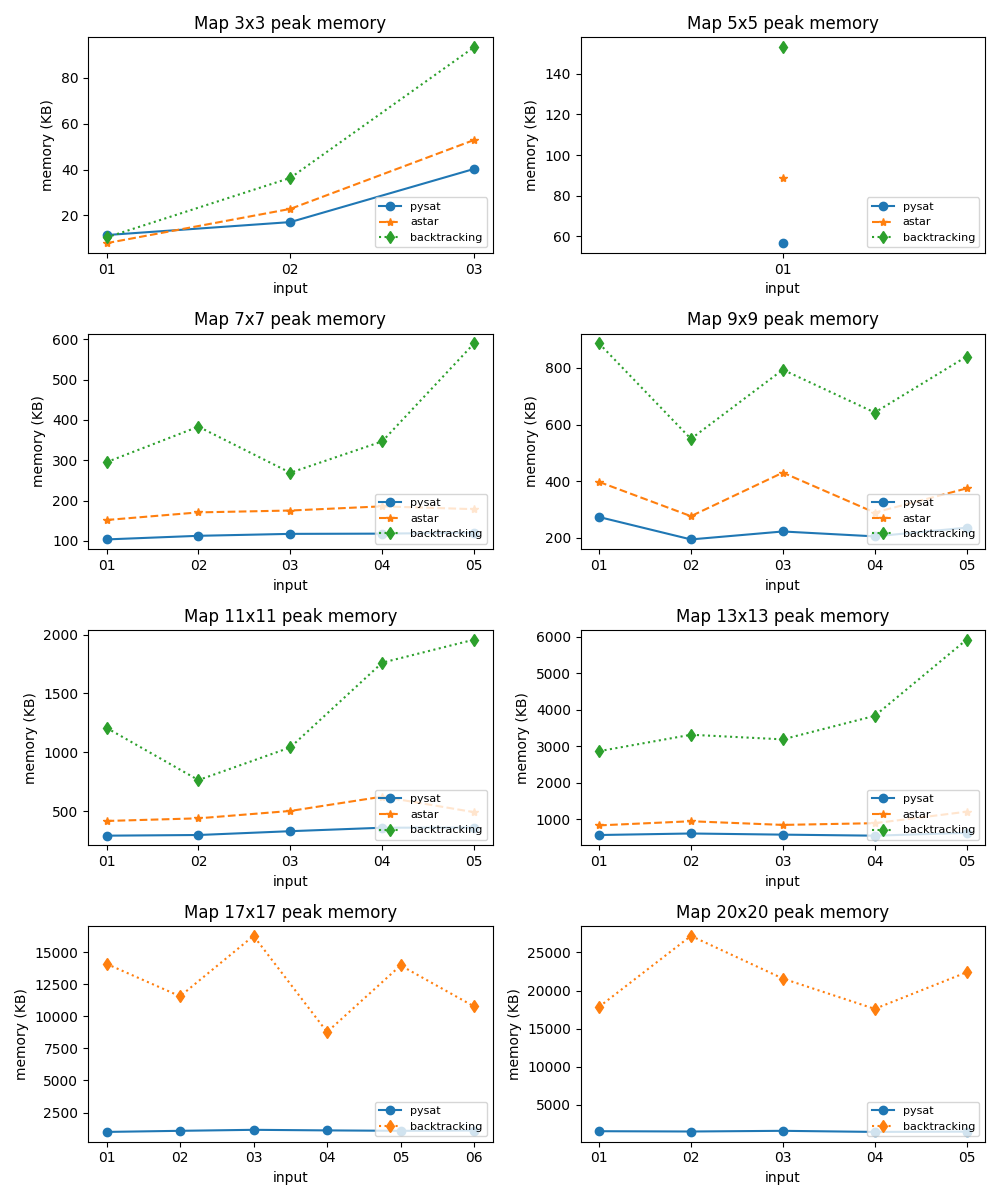
\includegraphics[width=0.95\textwidth]{imgs/benchmark-peak_memory.png}
    \caption{Solving time Benchmark}
\end{figure}


% References
\pagebreak
\section{References}
\begin{enumerate}
  \item \href{https://www.hashi.info/how-to-solve}{Hashi Info}: How to solve Hashiwokakero puzzles successfully (for human players)
  \item \href{https://en.wikipedia.org/wiki/Tseytin_transformation}{Tseytin Transformation}: About generating CNF clauses from DNF
\end{enumerate}
\end{document}
